% Бүлэг 3

\chapter{Системийн зохиомж, диаграм}
\label{Chapter3}
\section{Бүлгийн зорилго}
Энэ бүлэгт хүйсийн болон нийгмийн тэгш, хүртээмжтэй байдлыг хангахад чиглэсэн хиймэл оюунт чатбот зохиомжийг тодорхойлов. Системийн архитектур, үндсэн класс бүтэц, хэрэглэгчийн асуултад хариулах дараалал, баримт бичиг оруулах болон боловсруулах урсгал, байршуулалтын орчин, өгөгдлийн сангийн бүтэц, мөн аюулгүй байдал ба нууцлалын зохиомжийг тус тус авч үзсэн болно. Зохиомжийн үндэс нь Retrieval-Augmented Generation (RAG) аргачлал \cite{rag_survey} бөгөөд хариултыг мэдлэгийн санд тулгуурлуулан үүсгэх замаар хэлний загварын галлюцинацийн эрсдэлийг бууруулах зорилготой. \cite{hallucination_survey, ji_hallucination_survey}.

\section{Системийн ерөнхий архитектур}

Зураг \ref{fig:system-architecture}-д системийн ерөнхий архитектурыг харуулав. Хэрэглэгч веб интерфэйсээр дамжуулан асуултаа илгээх бөгөөд backend API нь хүсэлтийг \texttt{ChatService} хэсэг рүү дамжуулна. \texttt{ChatService} нь RAG pipeline-ыг ашиглан хэрэглэгчийн асуулттай хамааралтай баримт бичгийн хэсгүүдийг ChromaDB вектор сангаас \cite{chromadb} хайж, олдсон контекст мэдээллийг Google Gemini хэлний загварт \cite{gemini_report, gemini_api} дамжуулан эцсийн хариултыг үүсгэнэ.

Мэдлэгийн санд оруулах баримтуудыг урьдчилан, ажиллах орчноос гадуур (offline) дамжуулдаг бөгөөд \texttt{scripts/ingest.py} CLI хэрэгсэл нь баримт ачаалах, текст задлах, хэсэгчлэх, embedding үүсгэх, вектор санд хадгалах, мета өгөгдлийг өгөгдлийн санд бүртгэх үүрэгтэй. Embedding үүсгэх шатанд BAAI/bge-m3 олон хэлний шигтгээний загвар \cite{bge_m3}, дахин эрэмбэлэлтэд BAAI/bge-reranker-v2-m3 загвар \cite{bge_reranker} ашиглагдана. Ийнхүү ажиллах үед чатбот нь зөвхөн уншиж ажиллах горимтой бөгөөд хэрэглэгчийн асуултад зөвхөн ерөнхий хэлний загварын мэдлэгээр бус, эх сурвалжид тулгуурлан хариулт өгөх боломжтой болно.

\begin{figure}[H]
    \centering
    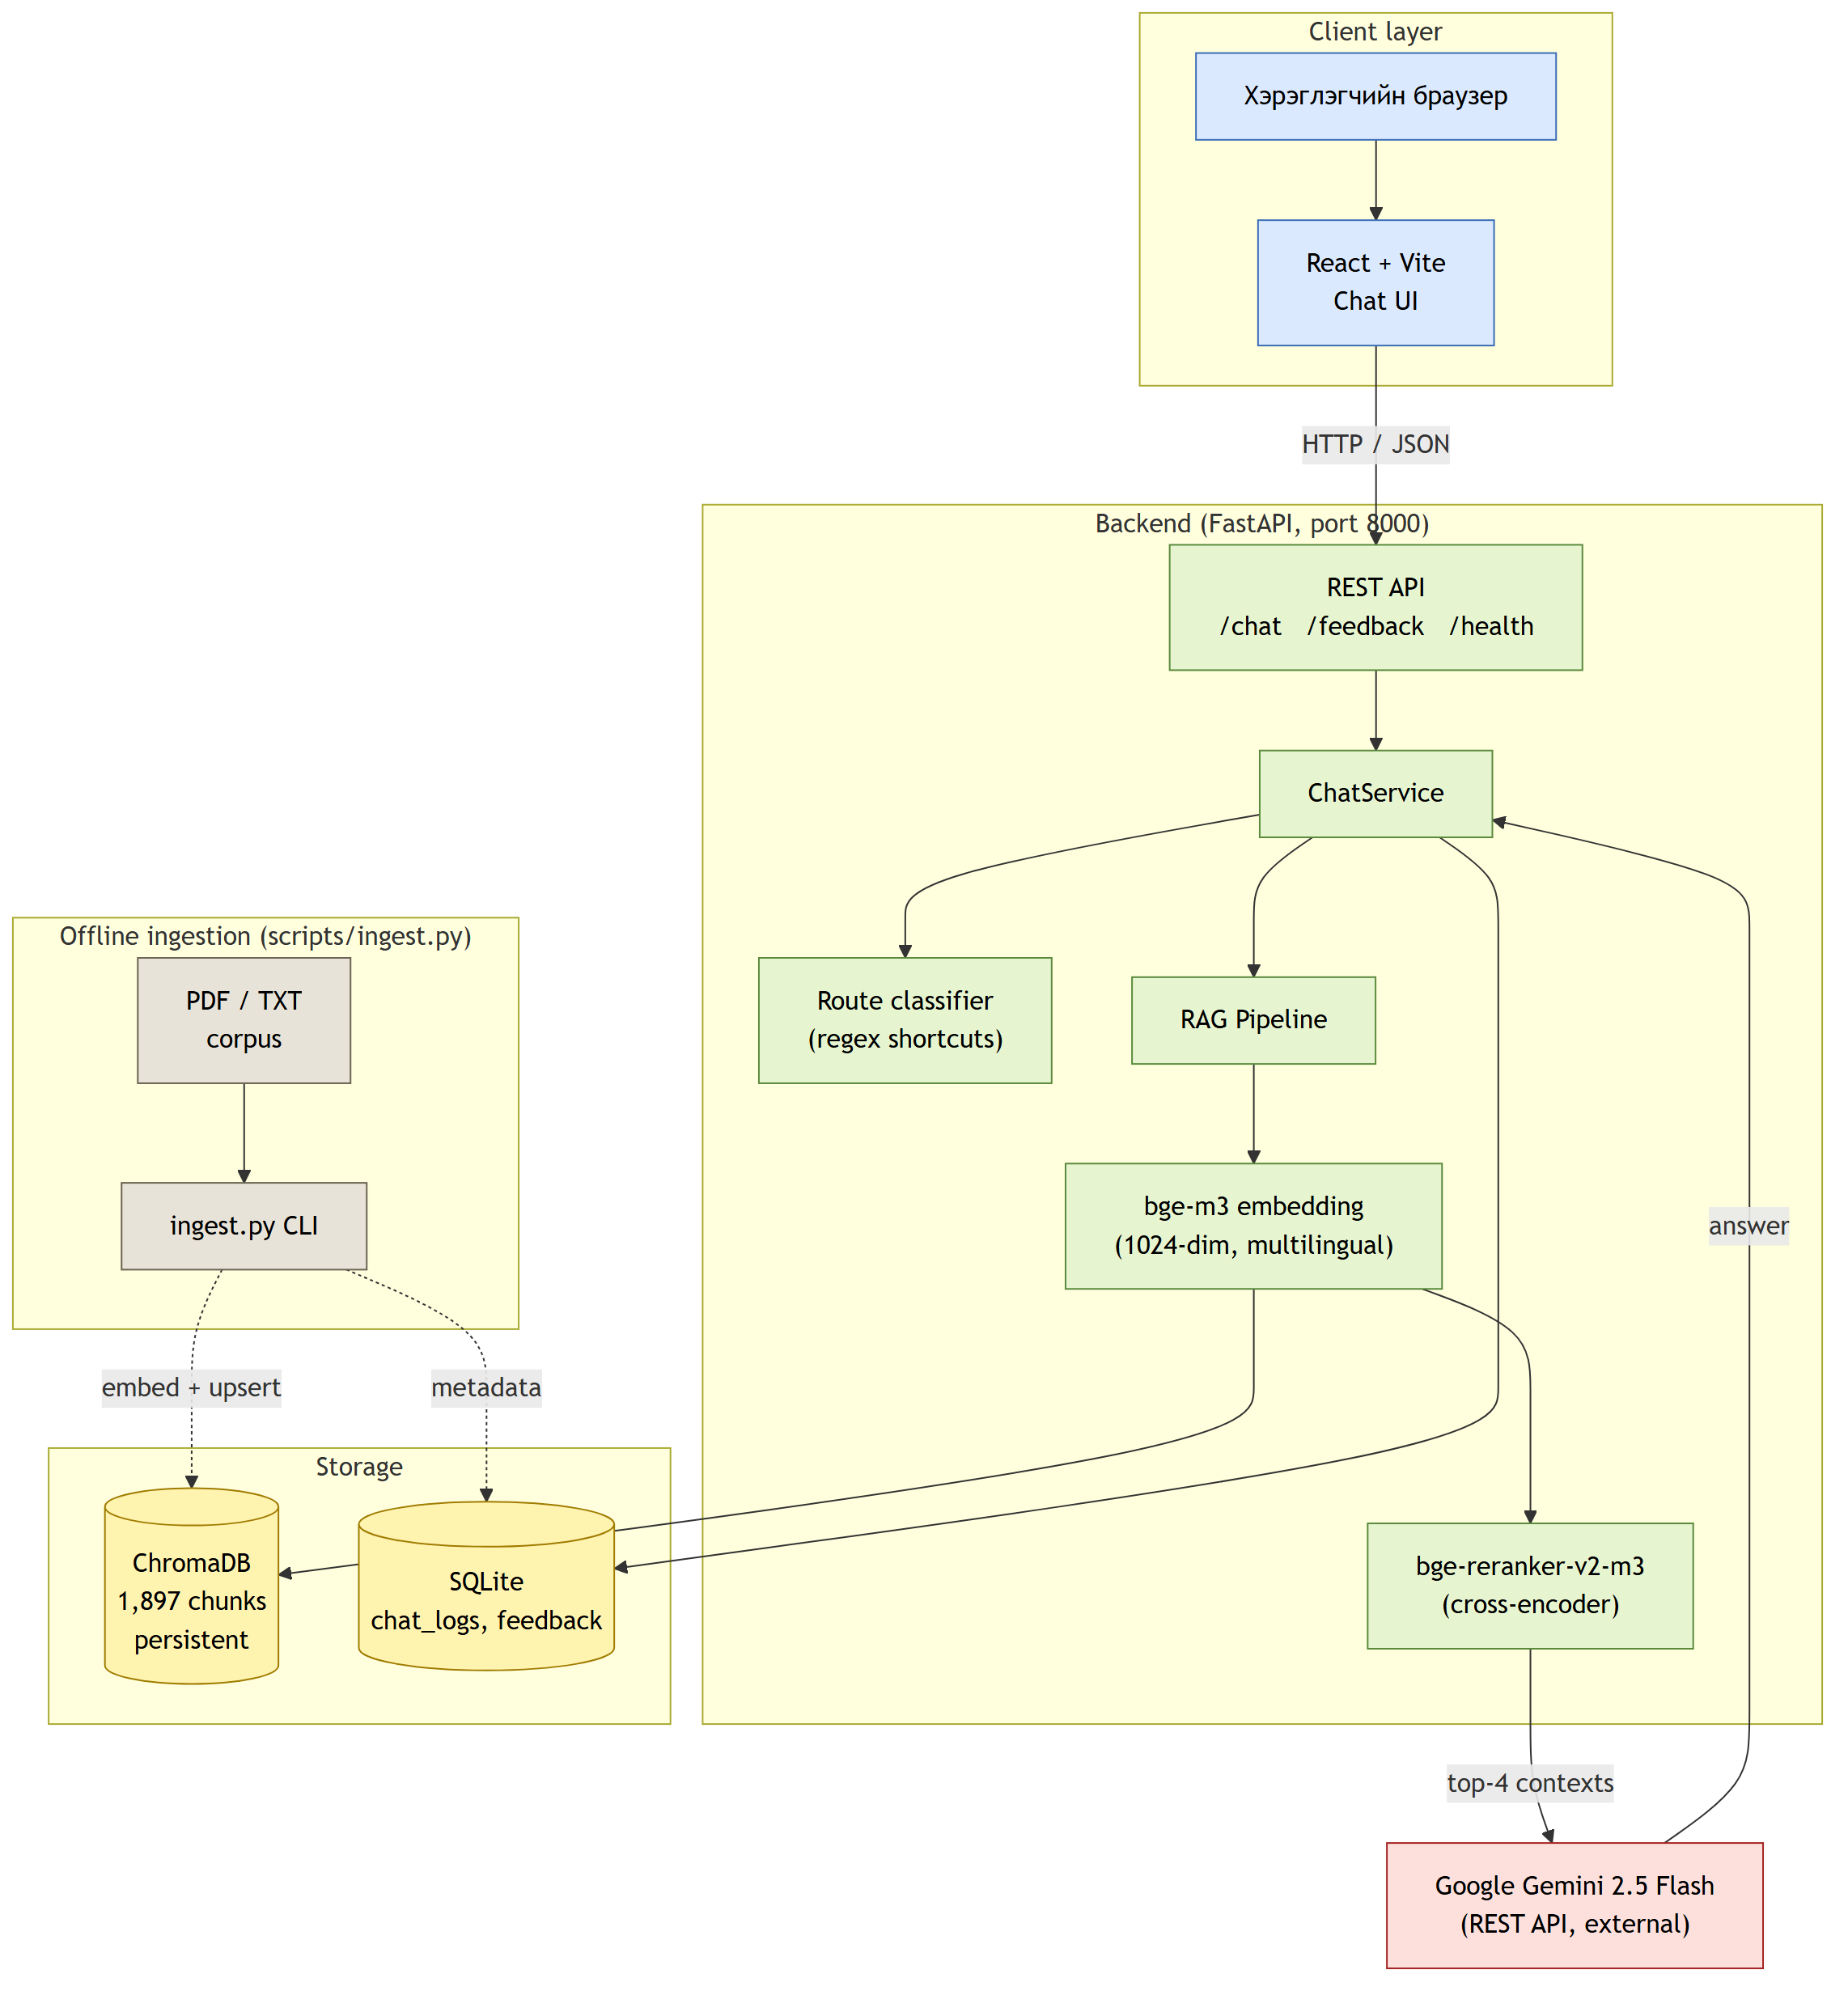
\includegraphics[
        width=1.1\textwidth,
        height=1.1\textheight,
        keepaspectratio
    ]{Diagrams/architecture.png}
    \caption[Системийн ерөнхий архитектур]{Системийн ерөнхий архитектур}
    \label{fig:system-architecture}
\end{figure}

\section{Архитектурын сонголтын үндэслэл}

Энэхүү системд RAG архитектурыг сонгосон гол шалтгаан нь байнга шинэчлэгдэх боломжтой баримт бичигт суурилсан хариулт өгөх шаардлагатай байсантай холбоотой \cite{rag_survey, grounded_generation}. Зөвхөн ерөнхий хэлний загварт тулгуурласан чатбот нь нарийвчилсан мэдээллийг шууд мэдэх боломжгүй бөгөөд эх сурвалжгүй зохиомол мэдээлэл үүсгэх эрсдэлтэй \cite{llm_limitations, hallucination_survey}. Харин RAG архитектур нь баримт бичгийг урьдчилан боловсруулж мэдлэгийн санд хадгалан, хэрэглэгчийн асуулттай хамгийн их хамааралтай хэсгийг хайж олдог тул илүү эх сурвалжид тулгуурласан хариулт үүсгэх давуу талтай.

Frontend хэсэгт React \cite{react_docs} болон Vite \cite{vite_docs}-ийг ашигласнаар хэрэглэгчийн интерфэйсийг уян хатан хөгжүүлэх боломж бүрдэнэ. Backend хэсэгт FastAPI \cite{fastapi}-ийг ашигласнаар API endpoint-уудыг асинхрон ажиллагаатай, өндөр гүйцэтгэлтэйгээр боловсруулах, Pydantic-д суурилсан өгөгдлийн шалгалт хийх, frontend болон AI pipeline хоорондын харилцааг зохион байгуулах боломжтой. Семантик хайлтын үе шатанд ChromaDB вектор санг \cite{chromadb} ашигласан бөгөөд энэ нь Python-д интеграц хийхэд хялбар, дискэнд тогтвортой хадгалагдах (persistent), мета өгөгдлийн шүүлтүүртэй хайлт дэмждэг давуу талтай. Шигтгээ үүсгэхэд олон хэлний BAAI/bge-m3 \cite{bge_m3} загвар, дахин эрэмбэлэлтэд BAAI/bge-reranker-v2-m3 \cite{bge_reranker} загварыг ашиглаж байгаа нь Монгол хэл болон бусад хэлэн дээрх хайлтын чанарт ач холбогдолтой. Хариулт үүсгэх хэсэгт Google-ийн Gemini 2.5 Flash хэлний загварыг \cite{gemini_report, gemini_api} REST API-р дамжуулан холбосон бөгөөд энэ нь олон хэл дэмждэг, контекстийн өргөн цонхтой, гүйцэтгэлийн зардал ба чанарын тэнцвэртэй сонголт юм. Реляц өгөгдлийн санд SQLite \cite{sqlite}-ийг ашигласан нь dependency багатай, бие даасан туршилтын орчинд тохиромжтой шийдэл болсон.

Архитектурын үндсэн давуу тал нь хэрэглэгчийн интерфэйс, backend API, баримт бичиг боловсруулах хэсэг, вектор хайлт болон хариулт үүсгэх хэсгүүдийг тус тусад нь салгасан явдал юм. Энэ нь системийг цаашид өргөтгөх, шинэ өгөгдөл нэмэх, хэрэглэгчийн интерфэйсийг өөрчлөх, эсвэл хэлний загварыг солих үед бүх системийг дахин бичихгүйгээр хэсэгчлэн сайжруулах боломжийг бүрдүүлнэ.

\subsection{Технологийн стек ба сонголтын үндэслэл}

Системд ашиглаж буй технологийн стекийг Хүснэгт~\ref{tab:tech-stack}-д нэгтгэн харуулав. Сонголт бүр нь нээлттэй эх, олон нийтийн дэмжлэгтэй, дипломын ажлын туршилтын хэмжээнд тохиромжтой, цаашид үйлдвэрлэлийн орчинд өргөтгөх боломжтой байх шалгуурыг хангадаг.

\begin{table}[H]
\centering
\footnotesize
\renewcommand{\arraystretch}{1.2}
\setlength{\tabcolsep}{4pt}
\begin{tabular}{|p{2.8cm}|p{3.5cm}|p{7.0cm}|}
\hline
\textbf{Бүрэлдэхүүн} & \textbf{Сонгосон технологи} & \textbf{Сонголтын үндэслэл} \\ \hline
Frontend & React 18 + Vite~\cite{react_docs,vite_docs} & Компонент суурьт UI, хөгжүүлэлтийн орчин хурдан, responsive веб интерфэйс бүтээх боломжтой \\ \hline
Backend API & FastAPI (Python)~\cite{fastapi} & REST API боловсруулахад хөнгөн бөгөөд хурдан, OpenAPI/Swagger баримт автоматаар үүсгэдэг, Pydantic validation дэмждэг. \\ \hline
Вектор сан & ChromaDB~\cite{chromadb} & Embedding вектор хадгалах, metadata ашиглан хайлт хийх, локал орчинд тогтвортой ажиллуулах боломжтой. \\ \hline
Embedding загвар & BAAI/bge-m3~\cite{bge_m3} & Олон хэл дэмждэг, dense, sparse болон multi-vector хайлтын аргыг хослуулдаг тул семантик хайлтад тохиромжтой. \\ \hline
Reranker загвар & BAAI/bge-reranker-v2-m3~\cite{bge_reranker} & Анхны хайлтаар олдсон top-$k$ үр дүнг дахин эрэмбэлж, хариултад ашиглах контекстийн чанарыг сайжруулна. \\ \hline
LLM & Google Gemini 2.5 Flash~\cite{gemini_report,gemini_api} & Олон хэл, урт контекст, хурдан хариу үүсгэх боломжтой бөгөөд API-р дамжуулан системтэй хялбар холбогдоно. \\ \hline
Реляц өгөгдлийн сан & SQLite~\cite{sqlite} & Тусдаа сервер шаардахгүй, локал орчинд ажиллахад хялбар, хэрэглэгчийн чат лог, тохиргоо болон санал хүсэлтийг хадгалахад тохиромжтой. \\ \hline
Тестлэлт ба баримт & pytest, OpenAPI & Backend service, RAG pipeline болон API endpoint-уудын ажиллагааг шалгах, API-ийн баримтыг автоматаар гаргах боломжтой. \\ \hline
\end{tabular}
\caption[Системийн технологийн стек]{Системийн технологийн стек ба сонголтын үндэслэл}
\label{tab:tech-stack}
\end{table}

\section{Өгөгдлийн сангийн бүтэц}

\section{Өгөгдлийн сангийн бүтэц}

Системийн өгөгдлийн сан нь баримт бичгийн мета өгөгдөл, боловсруулсан текстийн хэсгүүд, хэрэглэгчийн асуулт-хариултын түүх болон санал хүсэлт зэрэг мэдээллийг зохион байгуулалттай хадгалах зориулалттай. Үүнд SQLite өгөгдлийн санг ашигласан бөгөөд уг шийдэл нь тусдаа сервер шаардахгүй, локал орчинд хялбар ажиллах, жижиг болон дунд хэмжээний системийн өгөгдлийг найдвартай хадгалах давуу талтай.

Харин хэрэглэгчийн асуултад семантик хайлт хийхэд шаардлагатай embedding векторуудыг ChromaDB вектор санд \texttt{data/vectors/chroma/} замд persistent хэлбэрээр хадгална~\cite{chromadb}. Ингэснээр баримт бичгийн текстэн хэсгүүдийг зөвхөн уламжлалт түлхүүр үгээр бус, утгын ойролцоогоор хайх боломж бүрдэнэ.

Ийм бүтэц нь системийн өгөгдлийг хоёр түвшинд зохион байгуулах боломжийг олгоно. Нэгдүгээрт, SQLite нь бүтэцтэй өгөгдөл буюу баримт бичиг, чат лог, хэрэглэгчийн үнэлгээ зэрэг мэдээллийг хадгална. Хоёрдугаарт, ChromaDB нь embedding векторуудыг хадгалж, RAG pipeline-ийн retrieval үе шатанд ойролцоо утгатай текстийн хэсгийг хурдан хайж олоход ашиглагдана.

\begin{table}[H]
\centering
\begin{tabular}{|p{3.0cm}|p{10.3cm}|}
\hline
\textbf{Бүрэлдэхүүн хэсэг} & \textbf{Үүрэг} \\ \hline
Баримт бичгийн мэдээлэл & Системд оруулсан баримт бичгийн нэр, төрөл, байршил, оруулсан огноо болон эх сурвалжийн мэдээллийг хадгална. \\ \hline
Текстийн хэсэг буюу chunk & Баримт бичгээс задалж авсан жижиг хэсгүүдийн текст, эх сурвалжтай холбогдох мэдээлэл болон хайлтад ашиглагдах холбоосыг хадгална. \\ \hline
Вектор сан & Chunk бүрийн embedding векторыг хадгалж, хэрэглэгчийн асуулттай ойролцоо хэсгийг similarity search аргаар хайна. \\ \hline
Чатын түүх & Хэрэглэгчийн асуулт, системийн хариулт, ашигласан эх сурвалжийн мэдээллийг хадгалах боломжтой хэсэг юм.
\\ \hline
Санал хүсэлтийн мэдээлэл &
Хэрэглэгчийн өгсөн үнэлгээ, санал хүсэлт болон системийн хариултын чанарыг үнэлэхэд шаардлагатай мэдээллийг хадгална. \\ \hline
\end{tabular}
\caption[Өгөгдлийн сангийн бүрэлдэхүүн хэсгүүд]{Өгөгдлийн сангийн үндсэн бүрэлдэхүүн хэсгүүд}
\label{tab:database-structure}
\end{table}


Энэхүү өгөгдлийн зохион байгуулалт нь хэрэглэгчийн асуултад хариулах үед вектор сангаас холбогдох контекстийг хайж олох, харин баримт бичгийн эх сурвалж болон мета мэдээллийг өгөгдлийн сангаас сэргээх боломжийг бүрдүүлнэ. Цаашид системийг байгууллагын бодит орчинд ашиглах тохиолдолд хэрэглэгчийн эрхийн түвшин, audit log, chat history болон access control-той холбоотой хүснэгтүүдийг нэмэлтээр өргөтгөх боломжтой.

\section{RAG pipeline-ийн параметрүүд}

RAG системийн чанарт хамгийн их нөлөөлдөг хүчин зүйлс нь баримтыг хэсэгчлэх стратеги (chunking), embedding model, retrieval-ийн top-$k$ ба дахин эрэмбэлэлтийн (reranking) тохиргоо, мөн хариулт үүсгэлтийн температур юм \cite{rag_survey, dpr}. Хүснэгт~\ref{tab:rag-params}-д энэхүү системд тогтоосон үндсэн параметрүүдийг тэдгээрийн утга ба сонголтын үндэслэлийн хамт нэгтгэн харуулав.

\begin{table}[H]
\centering
\begin{tabular}{|p{3.4cm}|p{2.6cm}|p{7.9cm}|}
\hline
\textbf{Параметр} & \textbf{Утга} & \textbf{Үндэслэл} \\ \hline
Хэсгийн хэмжээ (chunk size) & 500 тэмдэгт & Утгын хувьд нэгэн цогц мэдээлэл хадгалах боломжтой бөгөөд хэт урт контекст үүсэхээс сэргийлнэ. \\ \hline
Хэсгийн давхцал (overlap) & 50 тэмдэгт & Хэсгүүдийн хоорондын утгын холбоог хадгалж, өгүүлбэр тасрах эрсдэлийг бууруулна. \\ \hline
Embedding загвар & BAAI/bge-m3~\cite{bge_m3} & Олон хэл, тэр дундаа Монгол кирилл текстийг дэмждэг, семантик хайлтад тохиромжтой өндөр чанартай загвар. \\ \hline
Embedding  dimensionality & 1024 & Embedding векторын илэрхийлэх чадвар өндөр бөгөөд утгын ялгааг илүү нарийвчлалтай хадгалах боломжтой. \\ \hline
Ижил төстэй байдлын хэмжүүр & Косинусын ижил төстэй байдал & Нормчилсон embedding векторуудын хоорондын утгын ойролцоог хэмжихэд тохиромжтой.~\cite{sentence_bert} \\ \hline
Retrieval Top-$k$ & $k=4$ & LLM-д дамжуулах контекстийн хэмжээг хязгаарлаж, хариултад ашиглах хамгийн хамааралтай хэсгүүдийг сонгоно. \\ \hline
Дахин эрэмбэлэх загвар(reranker) & BAAI/bge-reranker-v2-m3~\cite{bge_reranker} & Анхны хайлтаар олдсон үр дүнг дахин эрэмбэлж, хариултад ашиглах контекстийн чанарыг сайжруулна. \\ \hline
Хариулт үүсгэх загвар
(LLM) & Gemini 2.5 Flash~\cite{gemini_report} & Олон хэл дэмждэг, урт контекст боловсруулах боломжтой, API-р дамжуулан хурдан холбогдоно. \\ \hline
Температур & 0.15 & Бага температур нь хариултыг илүү тогтвортой, баримтад тулгуурласан, зохиомол хариулт үүсгэх эрсдэл багатай болгоно. \\ \hline
Хариултын дээд хэмжээ & 400 token & Хариултыг товч, ойлгомжтой байлгаж, prompt болон answer-ийн нийт токены хэрэглээг хянахад ашиглагдана. \\ \hline
\end{tabular}
\caption[RAG pipeline-ийн үндсэн параметрүүд]{RAG pipeline-ийн үндсэн параметрүүд ба сонголтын үндэслэл}
\label{tab:rag-params}
\end{table}

Эдгээр параметрүүд нь дипломын ажлын туршилтын орчинд тогтоогдсон утгууд бөгөөд цаашид үнэлгээний үр дүнд тулгуурлан системтэйгээр оновчилж болно. Тухайлбал retrieval-ийн чанарыг top-$k$ ба хэсгийн хэмжээтэй хамт хувьсгахад MRR ба recall@$k$ үзүүлэлтүүд хэрхэн өөрчлөгдөж буйг хэмжих замаар оновчтой утгыг олох боломжтой~\cite{dpr,ragas}.

\section{Класс диаграм}

Зураг \ref{fig:class-diagram}-д системийн үндсэн класс болон модулиудын хоорондын хамаарлыг харуулав. Класс диаграм нь frontend-ийн хуудас болон API client, backend-ийн router, service, repository, RAG pipeline, embedding service, vector store service, LLM service зэрэг гол бүрэлдэхүүн хэсгүүдийн уялдааг дүрсэлнэ.

Класс диаграмын зорилго нь системийн логикийг ямар хэсгүүдэд хуваан зохион байгуулсныг харуулах явдал юм. Жишээлбэл, хэрэглэгчийн асуултыг хүлээн авах хэсэг нь chat router-оор дамжиж, бизнес логик \texttt{ChatService}-д төвлөрнө. Харин баримт бичиг боловсруулах логик нь offline ingestion script-ээр дуудагдан document processor, embedding service, vector store service хэсгүүдээр дамжин хэрэгжинэ. Ингэснээр хэрэглэгчийн чат урсгал болон offline баримт бичиг боловсруулах урсгал хоорондоо ялгаатай боловч нэг мэдлэгийн сан дээр суурилан ажиллах боломжтой болно.

\begin{figure}[H]
    \centering
    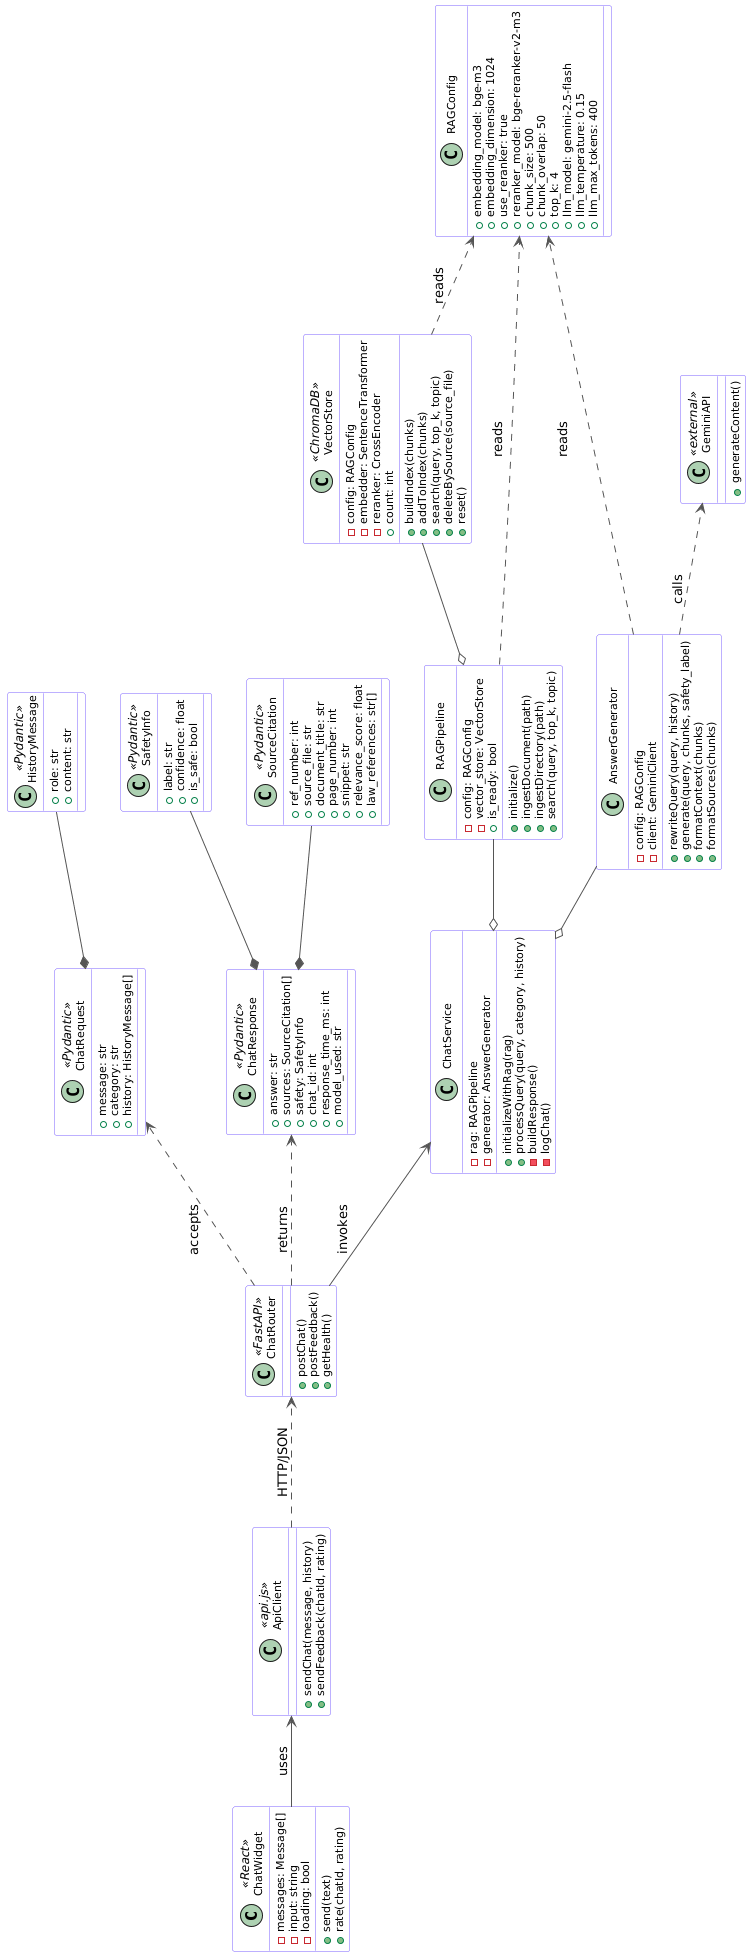
\includegraphics[
        width=1.1\textwidth,
        height=1\textheight,
        keepaspectratio
    ]{Diagrams/class5bosoo.png}
    \caption[Класс диаграм]{Системийн үндсэн класс диаграм}
    \label{fig:class-diagram}
\end{figure}


\section{Дарааллын диаграм}

Дарааллын диаграм нь системийн бүрэлдэхүүн хэсгүүд хоорондоо цаг хугацааны дарааллаар хэрхэн харилцаж байгааг харуулдаг. Энэхүү системийн хувьд хэрэглэгчийн асуултад хариулах урсгал болон offline баримт бичиг оруулах (corpus ingestion) урсгал гэсэн хоёр үндсэн дарааллыг авч үзэв.

\subsection{Асуулт хариултын дарааллын диаграм}

Зураг \ref{fig:sequence-answer-question}-д хэрэглэгч системд асуулт оруулснаас эхлэн эцсийн хариулт буцаж ирэх хүртэлх үндсэн дарааллыг харуулав. Хэрэглэгч асуултаа frontend хэсэгт оруулж, frontend нь backend API руу HTTP/JSON хүсэлт илгээнэ. Backend хүсэлтийг шалгасны дараа \texttt{ChatService} болон RAG pipeline руу дамжуулж, ChromaDB вектор сангаас холбогдох контекстийг хайна \cite{chromadb}. Олдсон контекстийг Google Gemini 2.5 Flash LLM-д дамжуулснаар хариулт үүсч \cite{gemini_api}, хэрэглэгчид буцаан харуулна.



\begin{figure}[H]
    \centering
    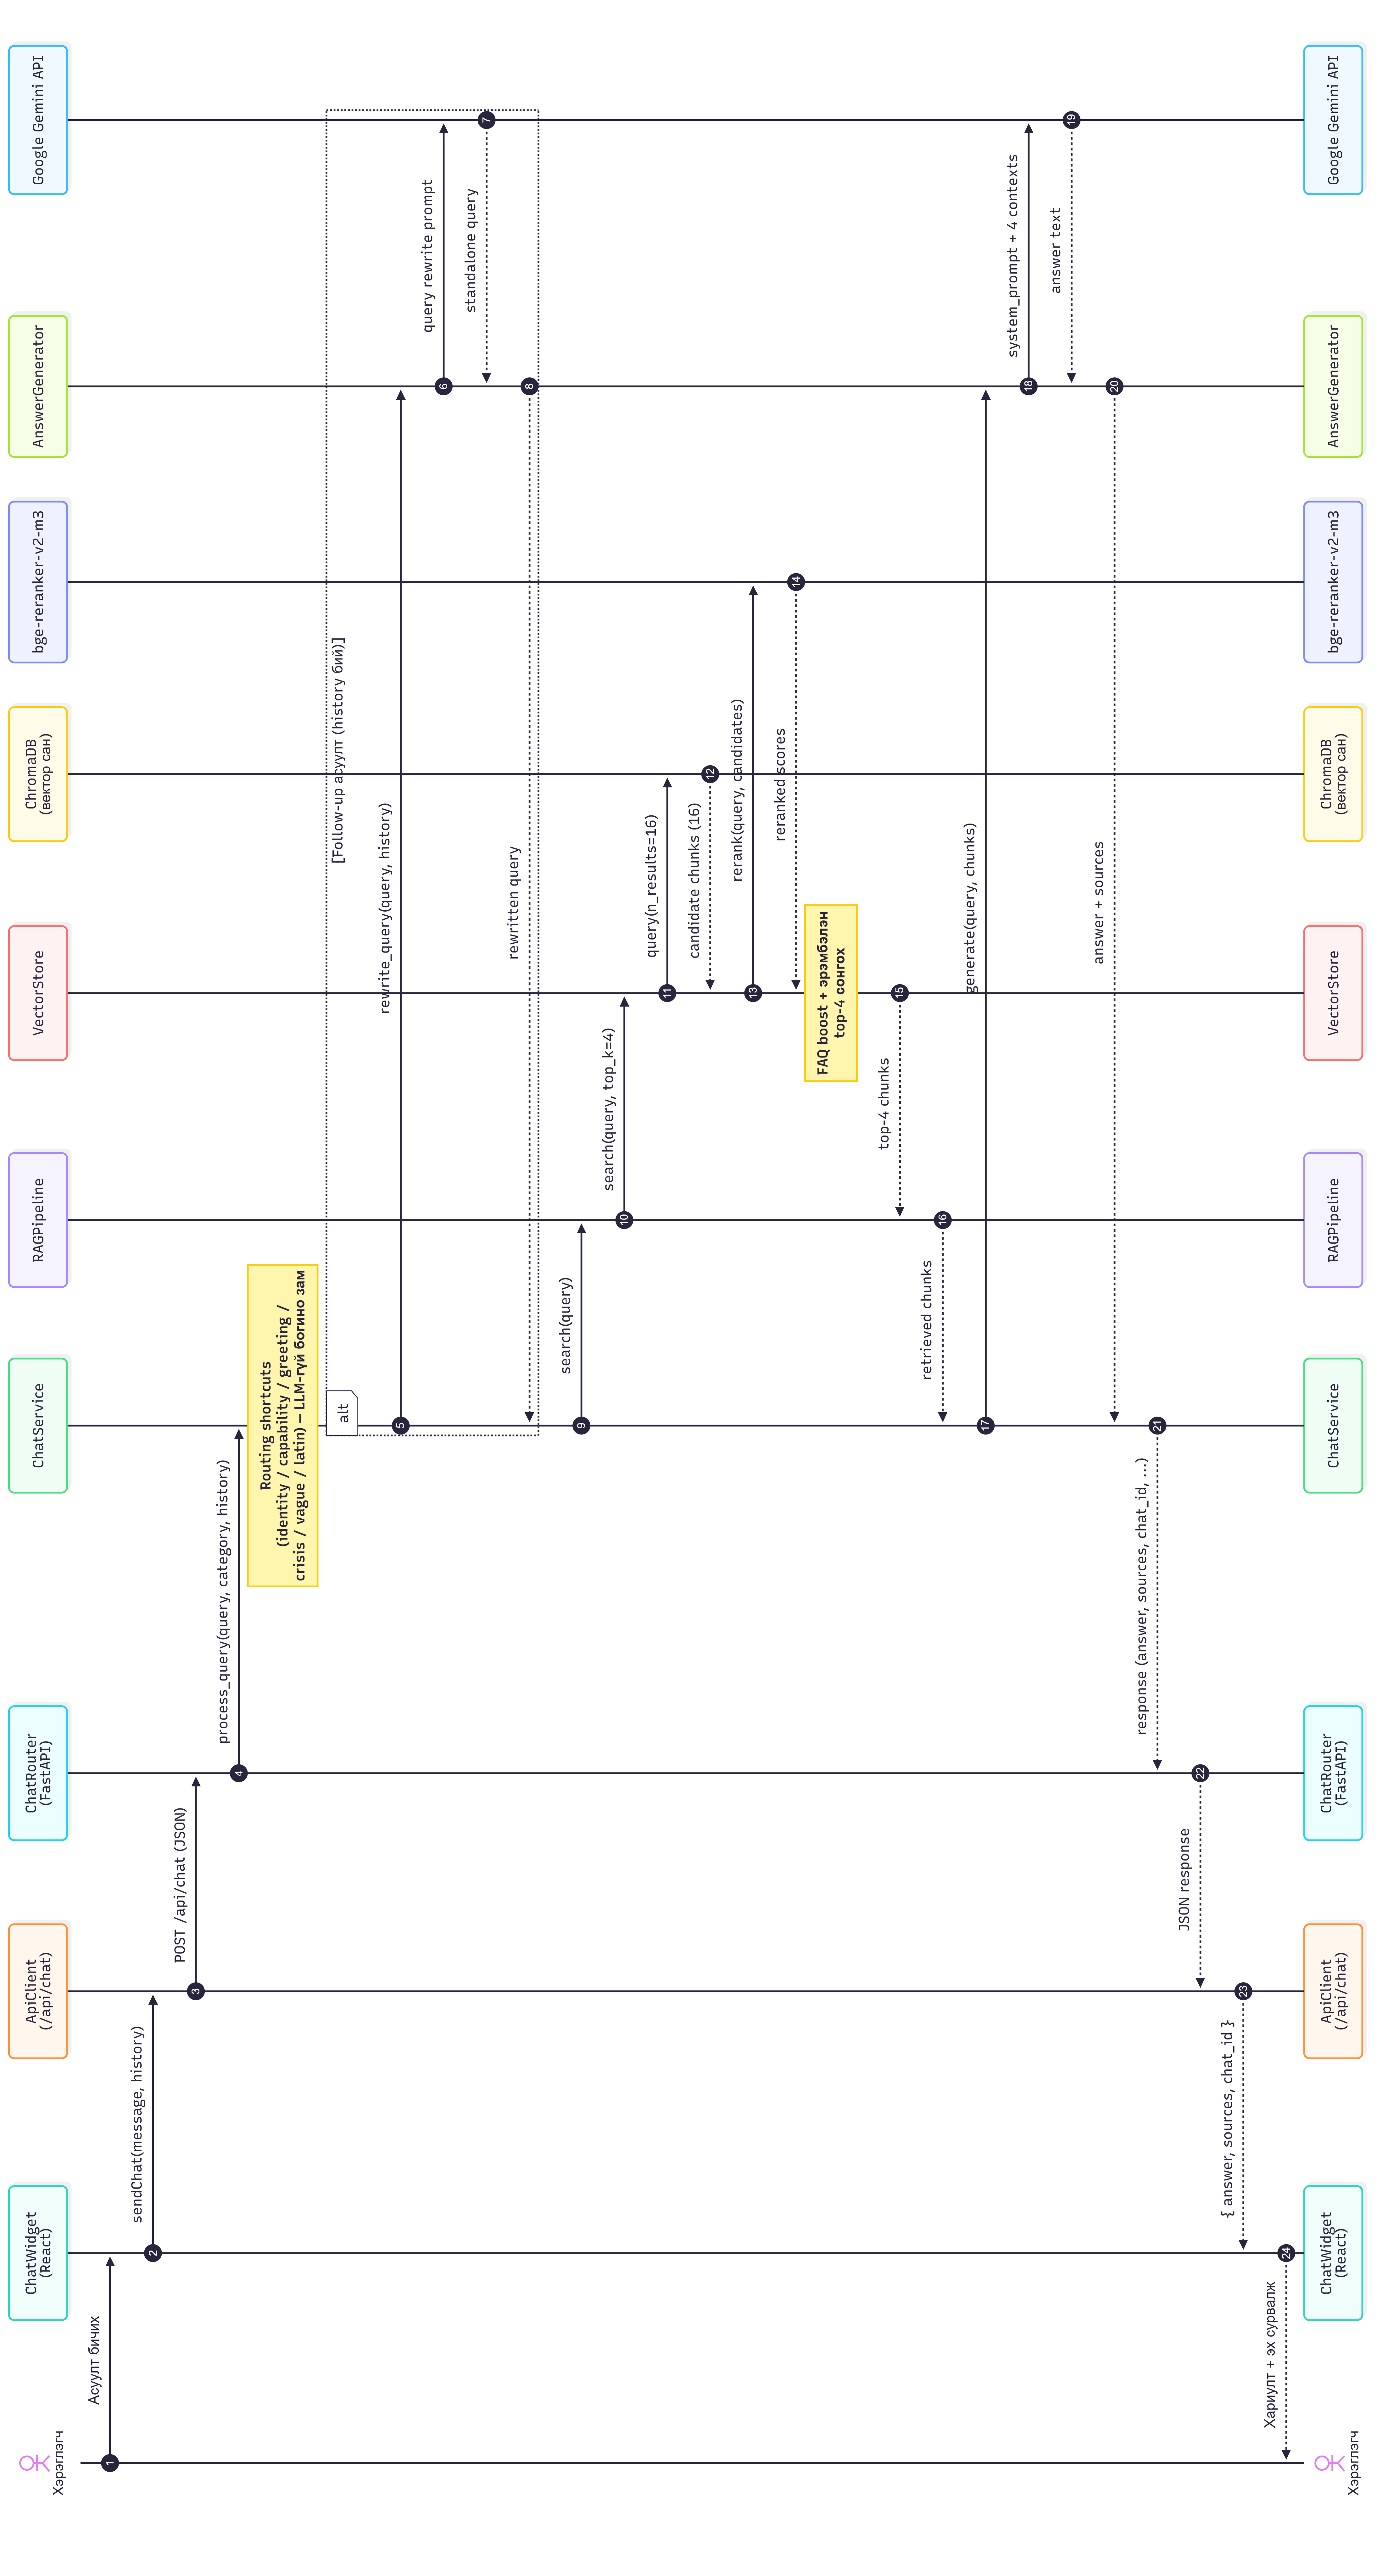
\includegraphics[
        width=1\textwidth,
        height=1\textheight,
        keepaspectratio
    ]{Diagrams/aq2.png}
    \caption[Асуулт хариултын дарааллын диаграм]{Асуулт хариултын дарааллын диаграм}
    \label{fig:sequence-answer-question}
\end{figure}

\subsection{Баримт бичиг оруулах дарааллын диаграм}

Зураг \ref{fig:sequence-document-upload}-д offline ingestion-ийн үед (\texttt{scripts/ingest.py} CLI хэрэгслээр) баримт бичиг оруулах үйл явцыг үзүүлэв. Хөгжүүлэгч/operator файлыг скриптэд дамжуулахад тухайн файлыг шалгаж, хадгалж, текст задлах процесс руу дамжуулна. Дараа нь задлагдсан текстийг хэсэгчилж, хэсэг бүрийн embedding үүсгэн вектор санд хадгална. Мөн баримт бичгийн нэр, эх сурвалж, үүссэн chunk-ийн мэдээлэл зэрэг мета өгөгдлийг өгөгдлийн санд бүртгэнэ. Энэхүү үйл явц нь системийн ажиллах үе шаттай хамааралгүй, зөвхөн corpus-ыг урьдчилан бэлдэхэд ашиглагдана.

\begin{figure}[H]
    \centering
    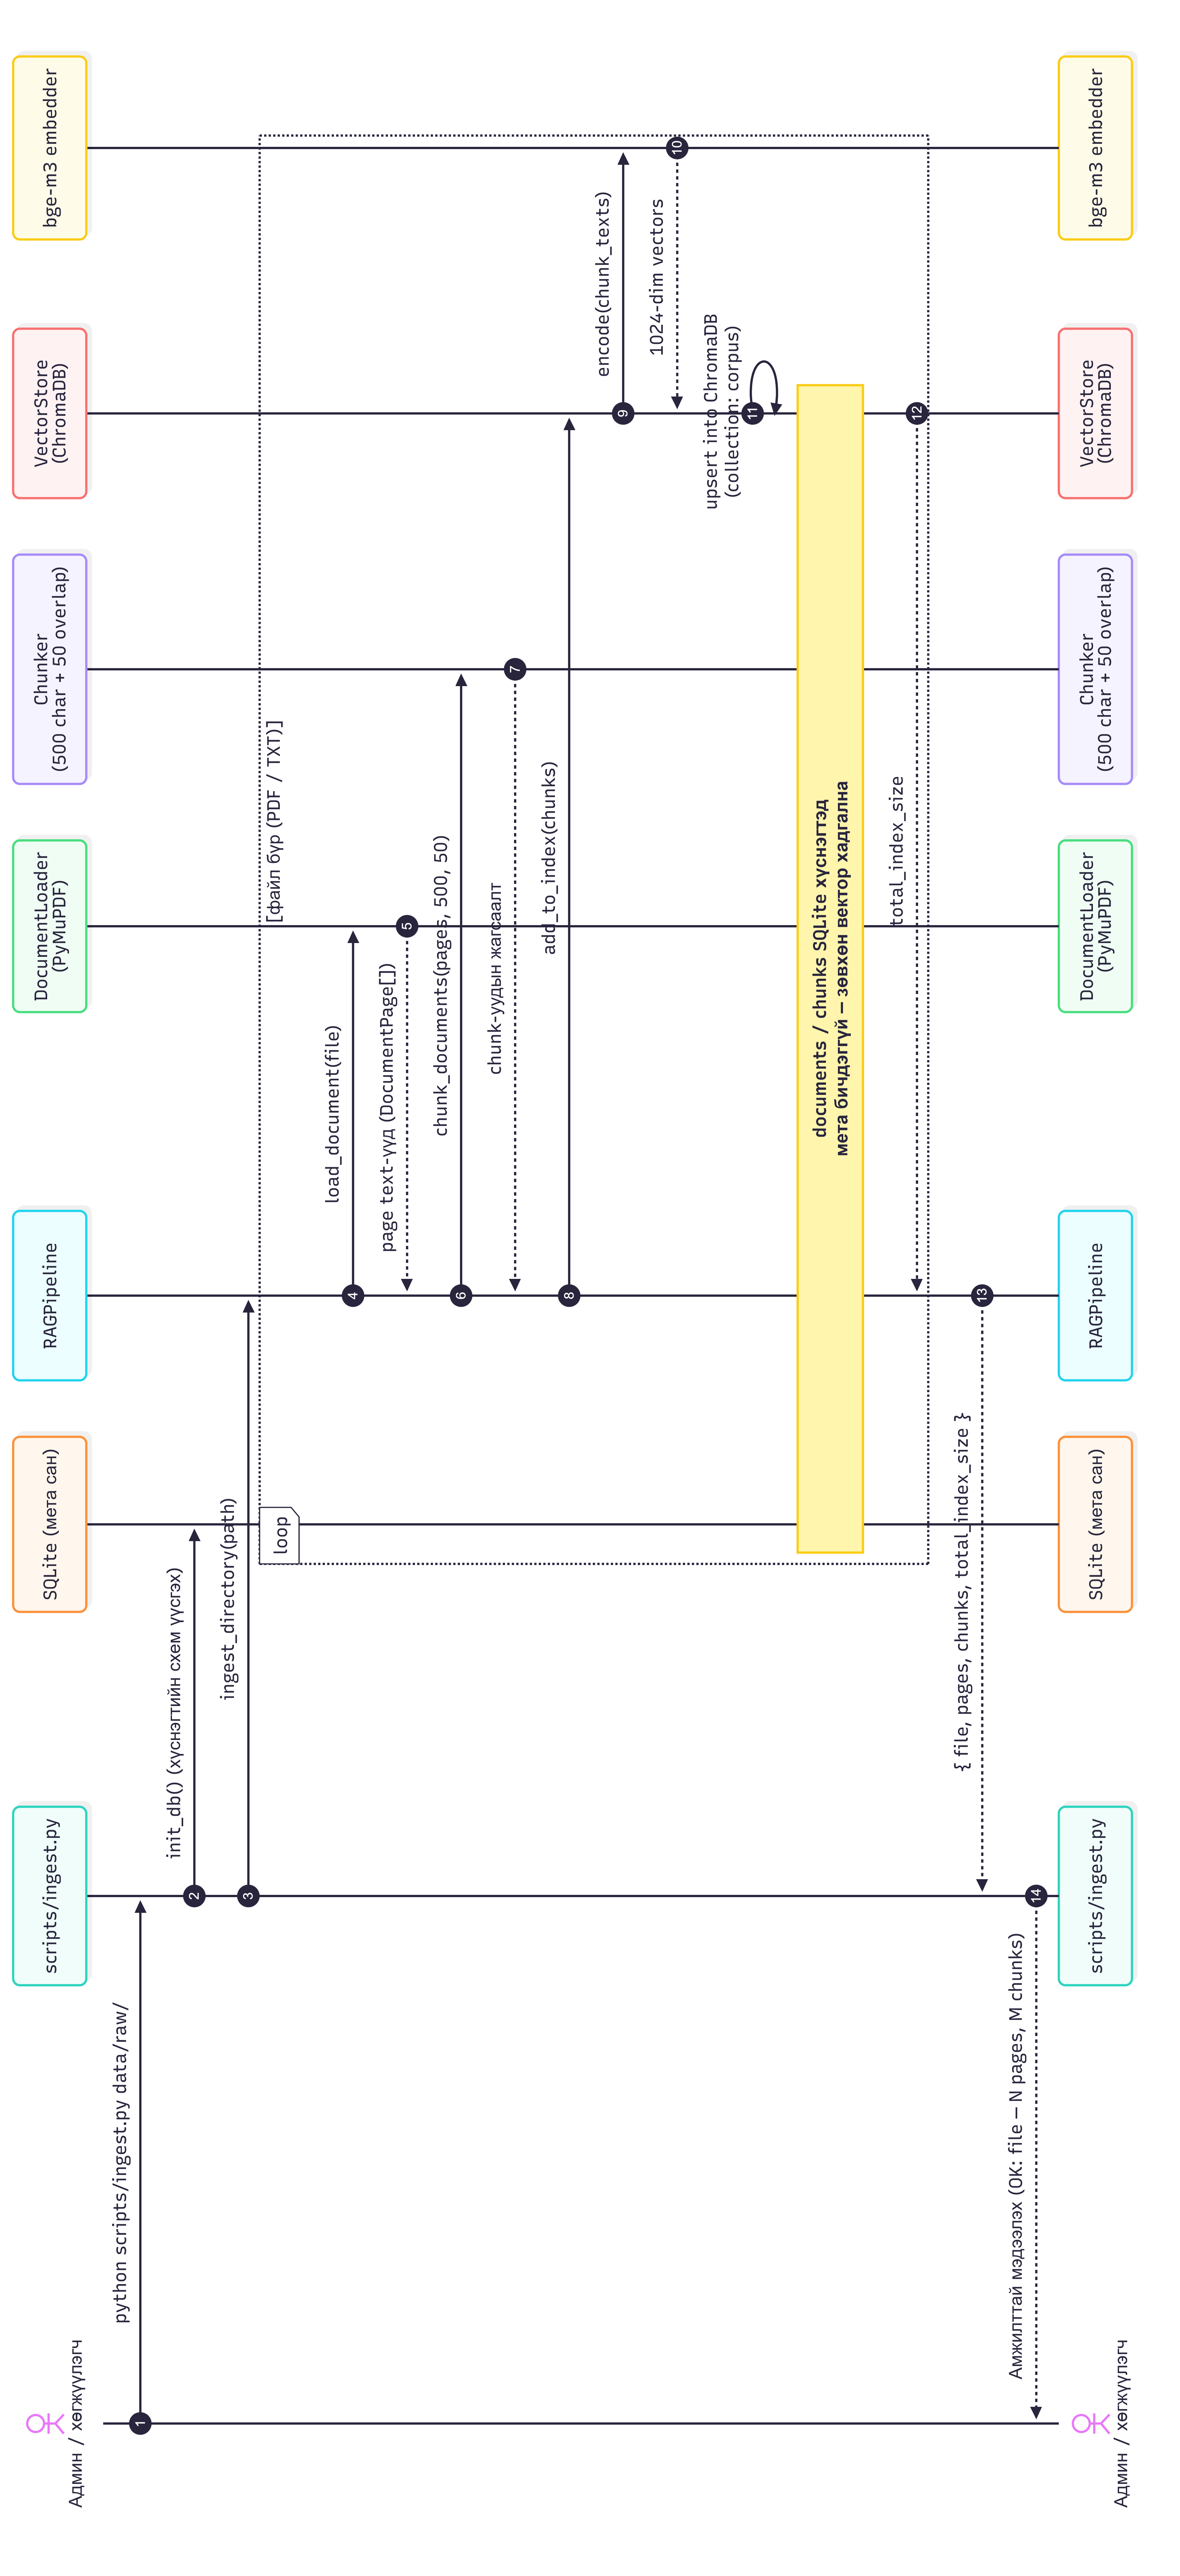
\includegraphics[
        width=1\textwidth,
        height=1\textheight,
        keepaspectratio
    ]{Diagrams/barimt2.png}
    \caption[Баримт бичиг оруулах дарааллын диаграм]{Баримт бичиг оруулах дарааллын диаграм}
    \label{fig:sequence-document-upload}
\end{figure}


\section{Байршуулах болон үйл ажиллагааны диаграм}

Энэ хэсэгт системийг ажиллуулах орчин болон баримт бичиг боловсруулах үйл ажиллагааны урсгалыг авч үзэв. Байршуулалтын диаграм нь хэрэглэгчийн браузер, frontend веб програм, FastAPI backend сервер, Gemini API, өгөгдлийн сан болон вектор сангийн хоорондын байрлал, харилцааг харуулна. Үйл ажиллагааны диаграм нь offline ingestion-ийн үед \texttt{scripts/ingest.py} систем дотооддоо ямар дарааллаар боловсруулалт хийдгийг тодорхойлно.

\subsection{Системийг байршуулах диаграм}

Зураг \ref{fig:deployment-diagram}-д системийн байршуулалтын ерөнхий орчныг харуулав. Хэрэглэгчийн браузер frontend веб програмтай харилцаж, frontend нь backend API руу хүсэлт илгээнэ. Backend нь Google Gemini API \cite{gemini_api} руу хариулт үүсгэх хүсэлт илгээж, SQLite өгөгдлийн сан \cite{sqlite}, ChromaDB вектор сан \cite{chromadb} болон raw documents хавтастай холбогдон ажиллана. Энэхүү зохион байгуулалт нь дипломын ажлын туршилт, demo үзүүлэх орчинд локал компьютер эсвэл сервер дээр ажиллуулахад тохиромжтой. Цаашид Docker container болон үүлэн орчинд (cloud) байршуулах боломжтойгоор зохион байгуулсан.

\begin{figure}[!htbp]
    \centering
    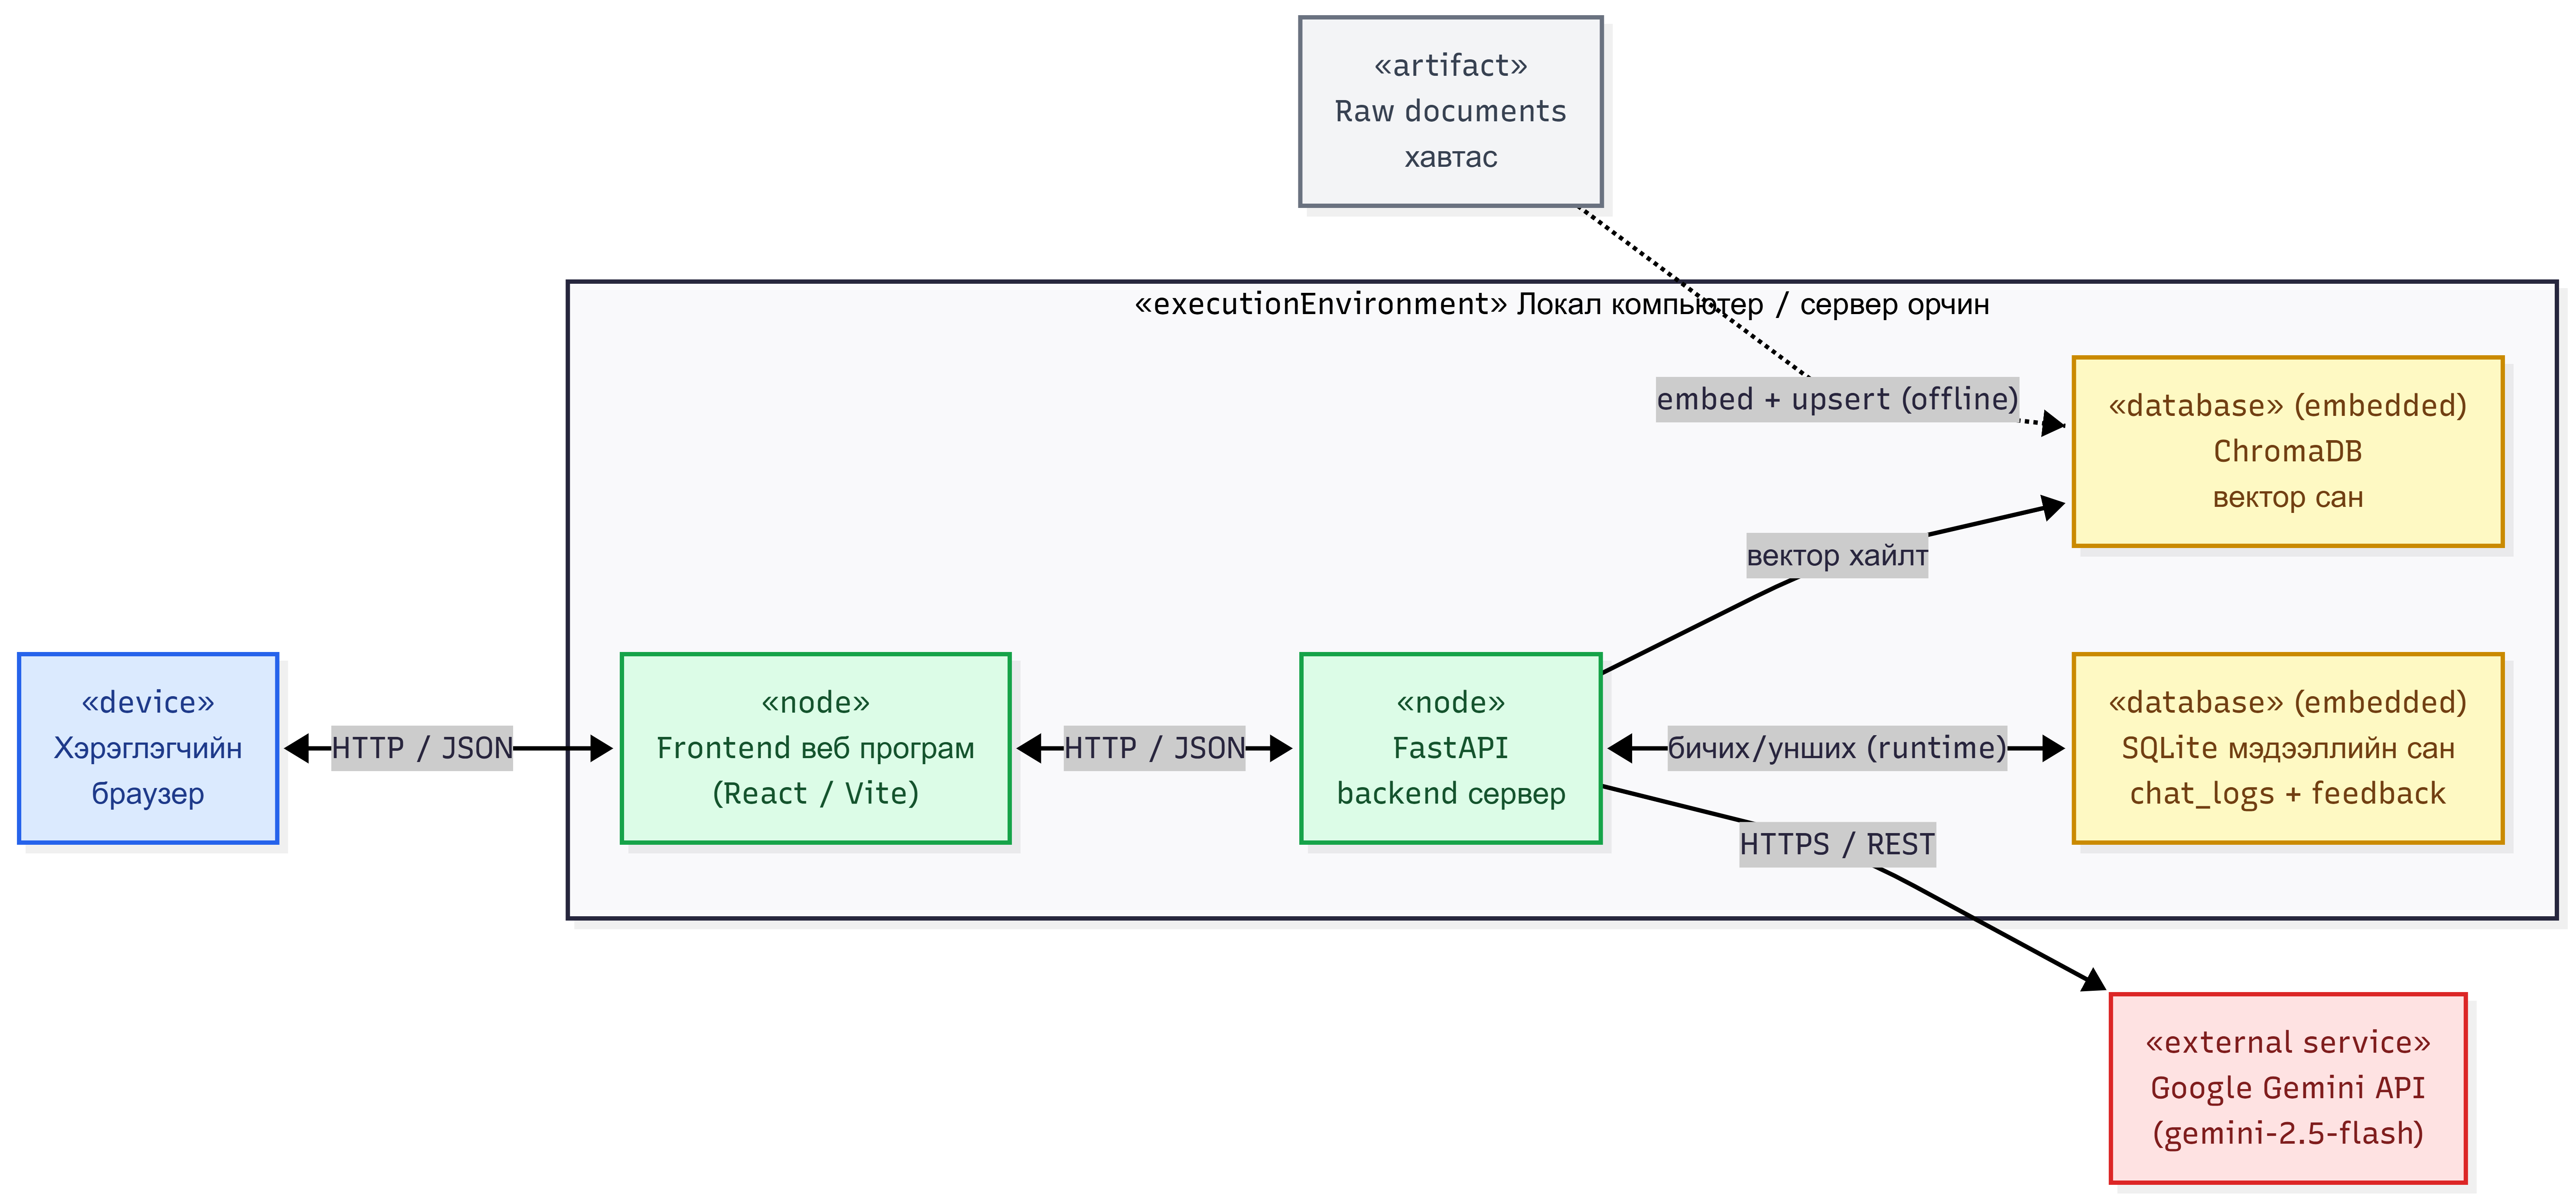
\includegraphics[
        width=1\textwidth,
        height=1.1\textheight,
        keepaspectratio
    ]{Diagrams/sysbairsh2.png}
    \caption[Системийг байршуулах диаграм]{Системийг байршуулах диаграм}
    \label{fig:deployment-diagram}
\end{figure}
\clearpage
\subsection{Баримт бичиг боловсруулах үйл ажиллагааны диаграм}

Зураг \ref{fig:document-processing-activity}-д баримт бичиг боловсруулах үйл ажиллагааны урсгалыг харуулав. \texttt{scripts/ingest.py} ingestion-д файлыг өгсний дараа систем тухайн файлыг хүчинтэй эсэхийг шалгана. Хэрэв файл шаардлага хангахгүй бол алдааны мэдээлэл буцаана. Харин хүчинтэй файл бол текст задлах, хэсэгчлэх, BAAI/bge-m3 загвараар embedding үүсгэх \cite{bge_m3}, ChromaDB вектор санд хадгалах \cite{chromadb}, SQLite-д мета өгөгдөл бүртгэх, индекс шинэчлэх гэсэн дарааллаар боловсруулагдана.

\begin{figure}[!htbp]
    \centering
    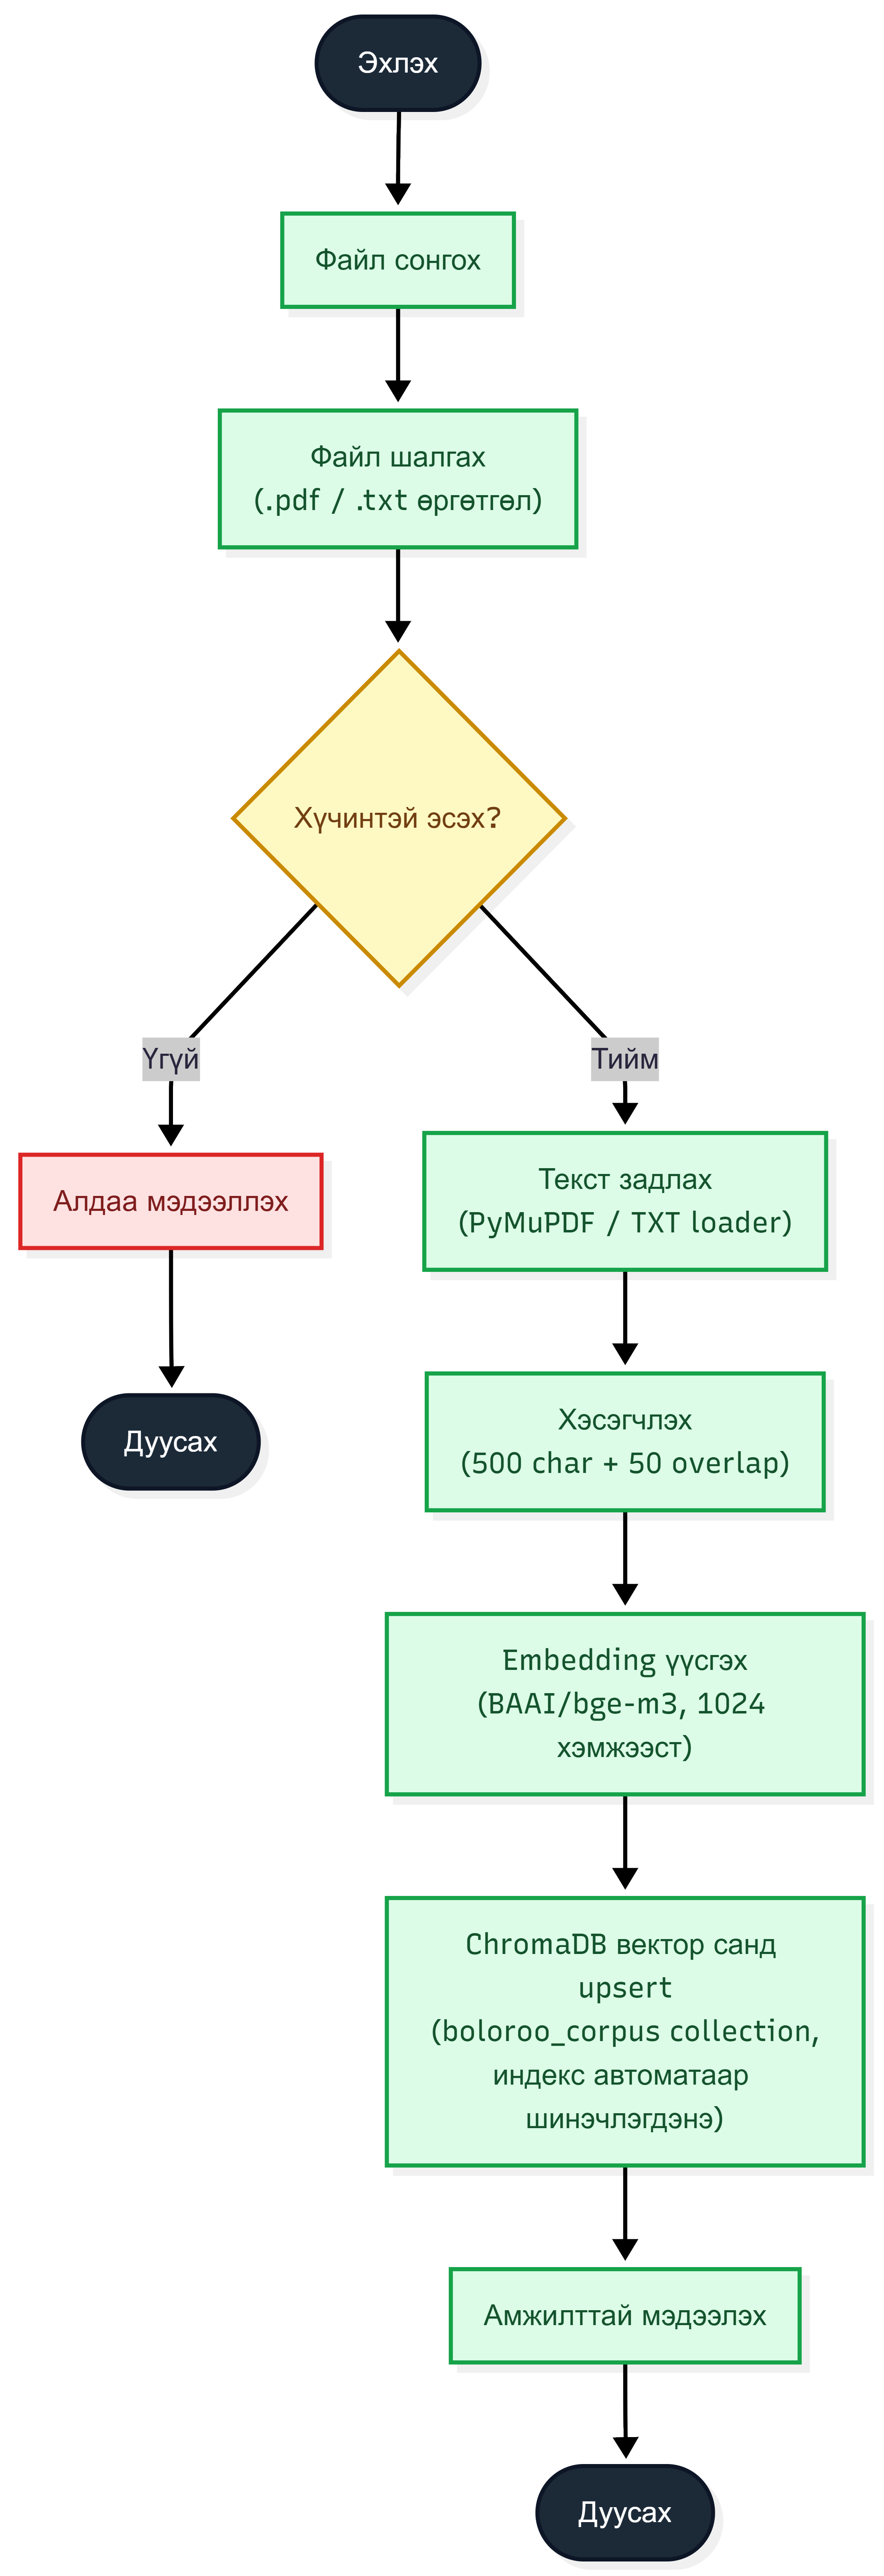
\includegraphics[
        width=1\textwidth,
        height=0.65\textheight,
        keepaspectratio
    ]{Diagrams/barimtbolovs2.png}
    \caption[Баримт бичиг боловсруулах үйл ажиллагааны диаграм]{Баримт бичиг боловсруулах үйл ажиллагааны диаграм}
    \label{fig:document-processing-activity}
\end{figure}

\section{Аюулгүй байдал ба нууцлалын зохиомж}

Тус системийн хэрэглэгчийн асуулт болон баримт бичиг нь зарим тохиолдолд байгууллагын дотоод бодлого, хувь хүний эрх, ажлын байрны мэдрэмжтэй асуудалтай холбоотой байж болно. Иймээс системийн зохиомжид өгөгдлийн нууцлал, хандалтын хяналт, баримт бичгийн эх сурвалжийн найдвартай байдал, хэрэглэгчийн мэдээллийг шаардлагагүйгээр хадгалахгүй байх зарчмыг харгалзан үзэх шаардлагатай. Энэхүү зохиомж нь Microsoft-ын Responsible AI зарчмууд \cite{responsible_ai}, NIST AI Risk Management Framework \cite{nist_ai_rmf} болон EU AI Act-ын ерөнхий чиглэлд \cite{eu_ai_act} нийцэхээр төлөвлөгдсөн.

Дипломын ажлын туршилтын хүрээнд хэрэглэгчийн өгөгдөл болон вектор санг локал орчинд хадгалах нь өгөгдлийг гадны үйлчилгээнд бүхэлд нь дамжуулах эрсдэлийг бууруулна. Хариулт үүсгэх Gemini API \cite{gemini_api}-руу зөвхөн хэрэглэгчийн асуулт болон retrieval-ээр сонгогдсон контекстийн хэсгийг илгээх бөгөөд бүх баримт бичгийн агуулга гаднын үйлчилгээ рүү дамждаггүй. Гэсэн хэдий ч бодит байгууллагын хэрэглээнд нэвтрүүлэх тохиолдолд өгөгдөл шифрлэлт, backup, audit log болон access control зэрэг нэмэлт хамгаалалтын механизмыг хэрэгжүүлэх шаардлагатай. Corpus-ыг урьдчилан бэлдсэн (offline) загвар нь runtime-д уншиж ажиллах горимтой бөгөөд document upload/delete-ийн API үргэлж байхгүй учир бодлогын баримтад зөвшөөрөлгүй өөрчлөлт оруулах эрсдэл багатай. Цаашид өгөгдлийн нууцлал илүү чухал болох тохиолдолд  (on-premise) хэлний загвар руу шилжих боломжтойгоор LLM-ийн интерфэйсийг хийсвэрлэн зохион байгуулсан.

Мөн чатботын хариултад жендэрийн хэвшмэл ойлголт, ялгаварлан гадуурхсан хэллэг, буруу зөвлөгөө үүсэхээс сэргийлэх шаардлагатай \cite{llm_limitations, hallucination_survey}. Иймээс prompt design, эх сурвалжийн чанар, хариултын хяналт, хэрэглэгчид өгөх анхааруулга зэрэг зохиомжийн элементүүдийг цаашид сайжруулах боломжтой. Системийн crisis-detection шат нь амь насанд аюул учруулах эрсдэлтэй илэрхийлэл (жишээ нь "амиа хорлох", "өөрийгөө гэмтээх" гэх мэт) илэрсэн тохиолдолд LLM-ийг алгасаж шууд тусламжийн утасны мэдээлэл буцаах байдлаар зохион байгуулагдсан бөгөөд энэ нь Responsible AI-ийн \textit{reliability and safety} зарчмын хэрэгжилт юм \cite{responsible_ai}.

\section{Бүлгийн дүгнэлт}

Энэ бүлэгт хүйсийн болон нийгмийн тэгш, хүртээмжтэй байдлыг хангахад чиглэсэн хиймэл оюунт чатбот системийн зохиомжийг тодорхойлсон. Системийн ерөнхий архитектур, архитектурын сонголтын үндэслэл, өгөгдлийн сангийн бүтэц, үндсэн класс диаграм, хэрэглэгчийн асуултад хариулах дараалал, баримт бичиг оруулах дараалал, системийг байрлуулах орчин болон баримт бичиг боловсруулах үйл ажиллагааны урсгалыг тус тус авч үзэв.

Систем нь хэрэглэгчийн асуултыг веб интерфэйсээр хүлээн авч, backend API-гаар дамжуулан RAG pipeline руу боловсруулалт хийдэг байдлаар зохион байгуулагдсан \cite{rag_survey}. RAG pipeline нь хэрэглэгчийн асуултад холбогдох баримт бичгийн хэсгүүдийг ChromaDB вектор сангаас \cite{chromadb} bge-m3 шигтгээгээр \cite{bge_m3} хайж, олдсон контекст мэдээллийг Google Gemini хэлний загварт \cite{gemini_report} дамжуулан эцсийн хариулт үүсгэх үндсэн зарчимтай. Ингэснээр чатбот нь зөвхөн ерөнхий мэдлэгт тулгуурлах бус, байгууллагын бодлого, дүрэм, заавар, сургалтын материал зэрэг баримт бичигт суурилсан хариулт өгөх боломжтой болж байна.

Мөн offline ingestion process-ийн талаас (\texttt{scripts/ingest.py}) баримт бичиг оруулах, текст задлах, хэсэгчлэх, embedding үүсгэх, ChromaDB вектор санд хадгалах, мета өгөгдлийг мэдээллийн санд бүртгэх үйл явцыг тодорхойлсон. Энэ нь системийн мэдлэгийн санг шинэчлэх, байгууллагын шинэ бодлого болон дүрэм журмыг системд нэмж ашиглах боломжийг бүрдүүлнэ.

Иймд энэхүү бүлэгт боловсруулсан системийн зохиомж нь дараагийн (4-р) бүлэгт авч үзэх хэрэгжүүлэлт, туршилт, үнэлгээний үндэс болж өгнө. Тодорхойлсон архитектур болон диаграмууд нь системийн бүрэлдэхүүн хэсгүүдийн үүрэг, өгөгдлийн урсгал, боловсруулалтын дараалал, байршуулалтын орчныг ойлгомжтой болгох бөгөөд дипломын ажлын программын шийдэл бодит систем хэлбэрээр хэрэгжих боломжтойг харуулж байна.
